\section{Analysis}
\label{sec:analysis}
The analysis technique is very simple;  Count the number of events in a cone drawn around the potential source, and determine if this number is consistent with the expected background of atmospheric neutrinos.  In order to choose the optimal opening angle for a galactic center search, a figure of merit is defined as Efficiency/$\sqrt{\textrm{Bckg}}$ for different cone half opening angles, using the signal MC described in Section \ref{sec:signal_mc} to compute the Efficiency for each cone and the official  SK atmospheric  MC for the number of events expected in the cone.  These figures of merit for cone half opening angles up to 40$^\circ$ are shown in Figure \ref{fig:opt_angle}.  In these figures of merit we care only about the shape not the magnitudes of the Efficiency/$\sqrt{\textrm{Bckg}}$, so the values for different models have been scaled by different amounts so that they can be seen together on the same plot.  As can be seen, the optimal angle ranges from $<5^\circ$ for NFW dark matter annihilation to $>40^\circ$ for Kravtsov dark matter decay.  Because of this, the analysis is performed with 8 different Galactic Center cone angles, ranging from $5^\circ$ to $40^\circ$ in steps of $5^\circ$.  For the solar search, the search is much more localized directionally, with the sun having an angular diameter of just ~0.5$^\circ$.  Therefore, a single cone with half opening angle of $5^\circ$ is used for the solar search.  


\begin{figure}
	\centering
	\subfigure[Annihilation]{
  	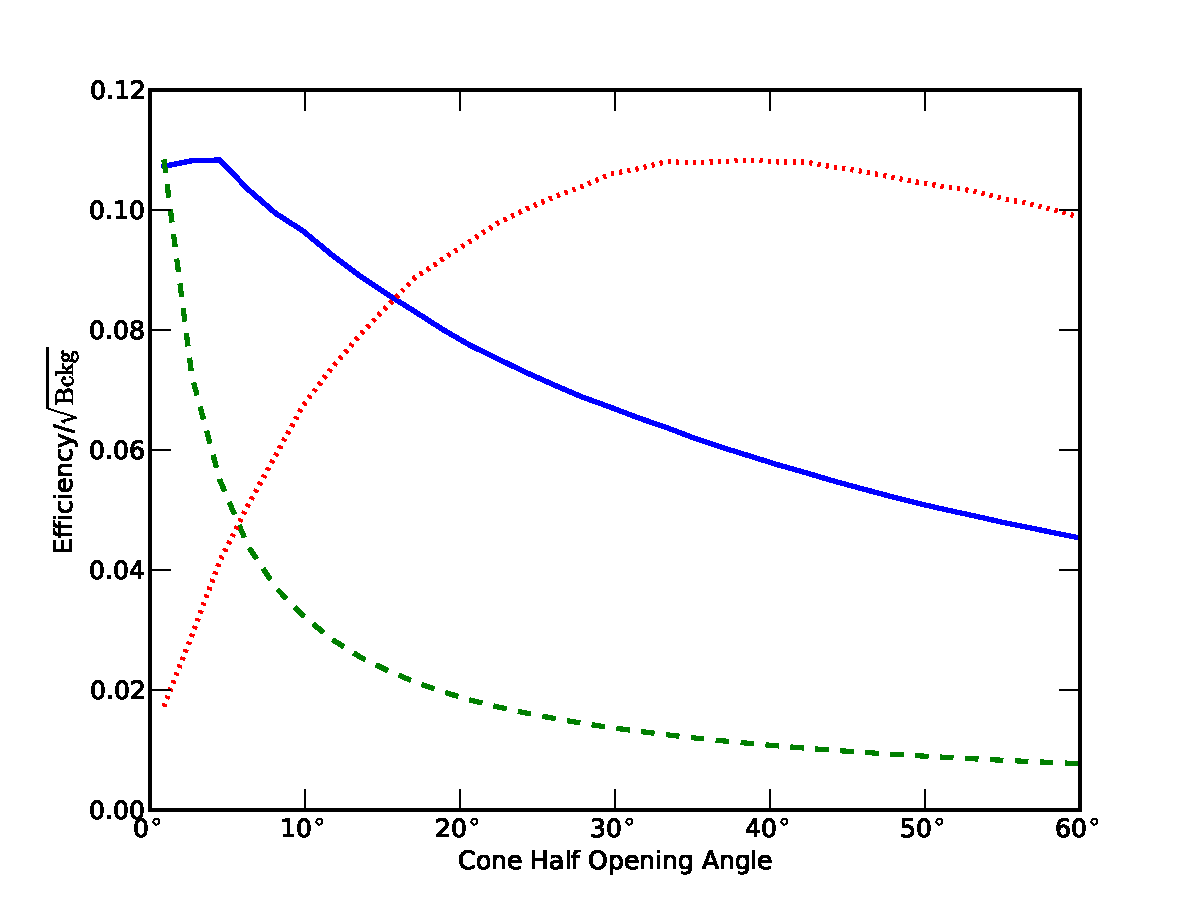
\includegraphics[width=0.4\textwidth]{figures/optimal_angle_ann.pdf}
	\label{fig:opt_angle_ann}
}
	\subfigure[Decay]{
	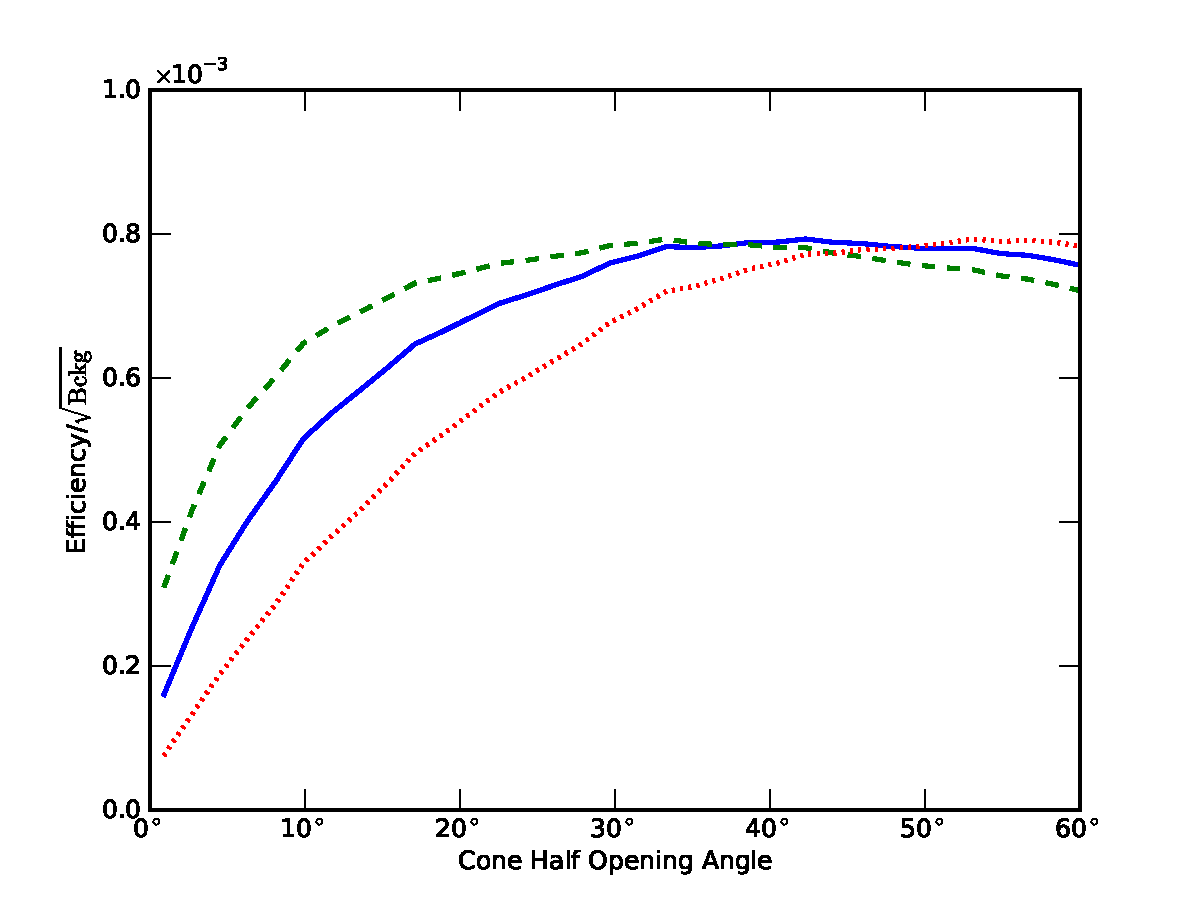
\includegraphics[width=0.4\textwidth]{figures/optimal_angle_d.pdf}
	\label{fig:opt_angle_d}
}
	\caption{Cone opening angle optimization for boosted dark matter from annihilation and decay.  In both \ref{fig:opt_angle_ann} and \ref{fig:opt_angle_d} the solid blue is the NFW halo model, dotted red is the Kravtsov halo model, and dashed green is the Moore halo model.  Note since the scaling is arbitrary, the efficiencies have been scaled by different amounts for each model so that they can all be seen on the same plot.}
	\label{fig:opt_angle}
\end{figure}





In order to quantify the agreement of the observed data with the background only or some level of excess signal hypothesis, a Poisson $\chi^2$ statistic is used which incorporates the systematic uncertainty of the background estimate using the pull method \cite{Fogli:2002do,Olive:2016xmw}:
\begin{equation}
\chi^2(s)=\min \limits_\epsilon\left[ 2  \left(  E -\mathcal{O}  + \mathcal{O} \ln \frac{ \mathcal{O} }{ E } \right)
             + \epsilon^2\right] \\
\label{eq:chi2}
\end{equation}
where,
\begin{equation}
E=b(1+\epsilon\sigma)+s
\end{equation} 
and $b$ is the estimated background with systematic uncertainty $\epsilon$, $s$ is the signal excess being tested, and $\mathcal{O}$ is the observed number of events.  The test statistic $\Delta \chi^2$ is calculated by subtracting from $\chi^2$ for the particular value of s the minimum $\chi^2$ for any value of s.  Note that this $\chi^2_\textrm{min}$ is easily computed as:
\begin{equation}
\chi^2_\textrm{min}=
\begin{cases}
0, & \textrm{if } b<=\mathcal{O} \\
\chi^2(0),& \textrm{if } b>\mathcal{O}
\end{cases}
\label{eq:x2_min}
\end{equation}
For each tested value of $s$, a large number of toy MC are produced.  If the fraction of toy MC produced with $\Delta \chi^2(s)$ less than the value found for the data is greater than or equal to $\alpha$, then s is excluded at $\alpha$ confidence \cite{Feldman:1998bu}.  

The minimization of $\chi^2$  over $\epsilon$ is done by setting
\begin{equation}    
\frac{\partial \chi^2}{\partial \epsilon}=2(b\sigma -\frac{\mathcal{O}b\sigma}{b(1+\sigma \epsilon)+s}) + 2\epsilon=0.
\label{eq:min_chi2_deriv}	
\end{equation}
Equation \ref{eq:min_chi2_deriv} leads to a simple quadratic equation with solutions
\begin{equation}
\epsilon=\frac{-(b\sigma^2+1+s/b) \pm \sqrt{(b\sigma^2+1+s/b)^2-4\sigma(b\sigma+\sigma s-\mathcal{O}\sigma)}}{2\sigma}.
\label{eq:quad_eq}
\end{equation}

Both solutions to Equation \ref{eq:quad_eq} are tested, and the smaller of the two resulting $\chi^2$ values is taken as the correct $\chi^2$.  Note that if $\epsilon<-1/\sigma$, which would imply pulling the background to a negative value, then $\epsilon$ is set to $-1/\sigma$ so that the background is pulled to 0.  Generally this would only happen for Data and MC which agree very poorly with a large systematic uncertainty, however it must be accounted for since it could occur a small number of times over many toy MC samples.

\subsection{Trials Factors}
\label{sec:trials_factors}
The correlations between the 8 galactic center cones (the smaller cones are subsets of the larger cones) leads to complicated trials factors when trying to understand the significance of any excess.  In order to understand the trials factors, 250,000 toy mc ensembles were created for both low and medium energy samples.  For each energy range, 8 bins in $\cos \theta_{\textrm{GC}}$ of width $5^\circ$ are shifted by a single shared systematic error for that energy range, chosen from a random Gaussian distribution with width given by the systematic uncertainties computed in Section \ref{sec:background_estimation}.  From the expected background, the number of toy mc events in each bin is then chosen as a Poisson random variable.  The number of events in each of the 8 cones around the galactic center is then calculated for the toy mc ensemble by adding up the events in the bins contained in each cone.  The significance of any excess in each cone is computed as described above, and the largest excess out of the 8 cones is recorded.  The probability that at least 1 of the 8 cones finds an excess of a particular significance $\alpha$ is then calculated, which allows for the adjustment of the significance to include the trials factor.  The results of this study are shown in Figure \ref{fig:trials_factors}.    Note that the results fall between the expectations for 8 perfectly correlated or 8 completely uncorrelated measurements.

\begin{figure}
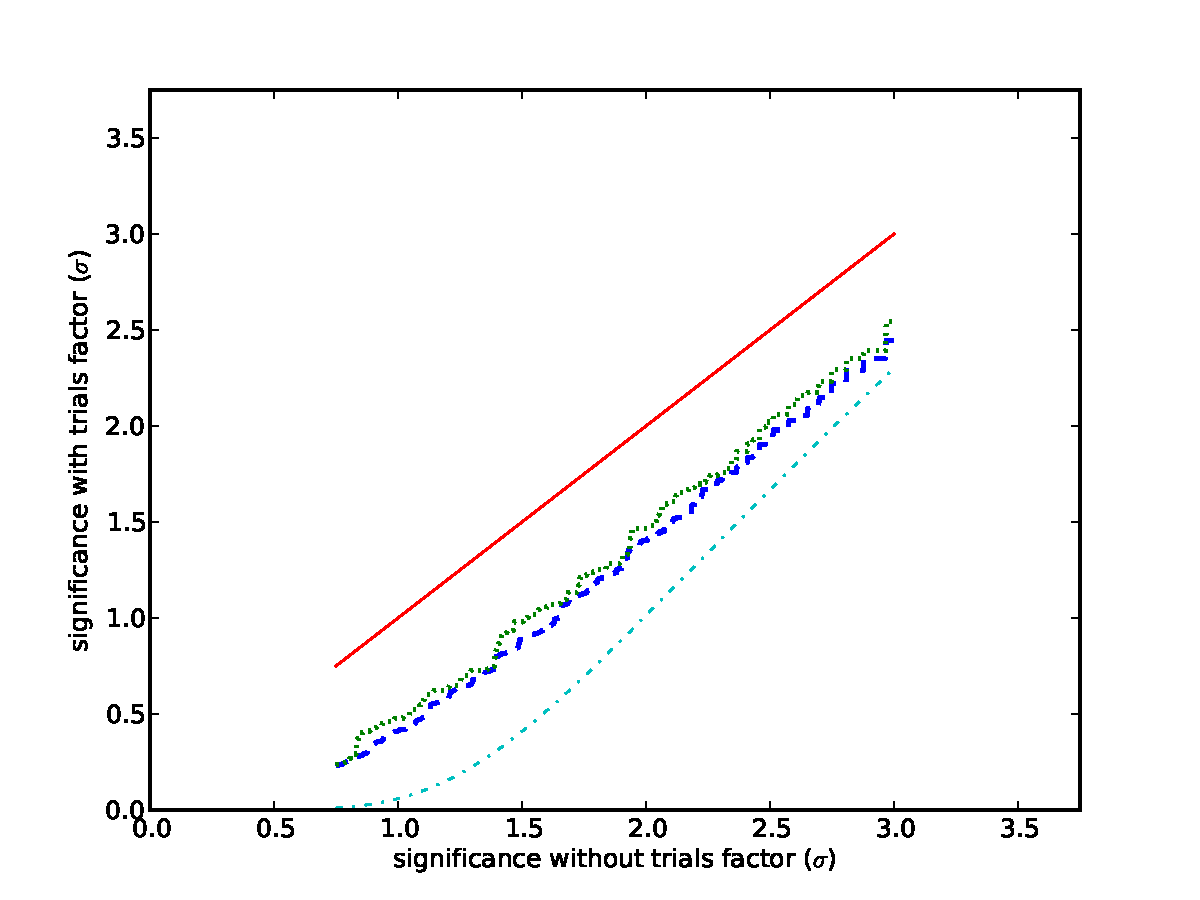
\includegraphics[width=0.45\textwidth]{figures/trial_factors.pdf}
\caption{Trials factor effect. The dashed blue (dotted green) line converts the significance of an excess without the trials factor included into the significance with the trials factor included for the low (medium) energy sample, based on Toy MC.  As reference, the solid red line shows y=x, the conversion for perfectly correlated measurements, and the dashed-dotted cyan line shows the conversion for 8 uncorrelated measurements.  Note that the effect for the galactic center cones falls between the perfectly correlated and perfectly uncorrelated effects, as expected.}
\label{fig:trials_factors}
\end{figure}   

\subsection{Limits on a simple Model}
\label{sec:limits_simple_model}
Reference \cite{Agashe:2014yua} presents a baseline boosted dark matter model.  In this model, a heavy dark matter particle A is the dominant dark matter of the universe.  This particle A does not couple directly to standard matter, but instead annihilates into a lighter dark matter particle B, which couples to standard matter through the exchange of a dark photon $m_{\gamma '}$, as in \cref{fig:feyn}.  The relic abundance of A is determined by an assisted freeze out scenario, and the thermal cross section is set to $\langle \sigma_{A\bar{A} \rightarrow B\bar{B}} \rangle=5 \times 10^{-26}$ cm$^3$/s in order to achieve the observed relic density $\Omega_A \approx 0.2$ \cite{Agashe:2014yua}.  The flux of boosted dark matter from the galactic center is 
\begin{equation}
\frac{d\Phi}{d\Omega dE_B}=\frac{1}{2}\frac{r_\textrm{sun}}{4\pi} \left(\frac{\rho_\textrm{local}}{m_A}\right)^2\mathcal{J}\langle \sigma_{A\bar{A} \rightarrow B\bar{B}} \rangle\delta(E_B-m_A).
\label{eq:flux}
\end{equation}
Note that any adjustment to the thermal cross section simply results in a corresponding scaling of the limits on $\sigma_{Be^- \rightarrow Be^-}$ found in \cref{sec:results}.  


\begin{figure}

\centering
\subfigure[Annihilation $A\bar{A} \rightarrow B\bar{B}$]{
\begin{tikzpicture}
\begin{feynman}
\vertex (b) [blob] at (0,0){};
\vertex (i1)[above left=of b] {A};
\vertex (i2)[below left=of b] {$\bar{A}$};
\vertex (f1)[above right=of b] {B};
\vertex (f2)[below right=of b] {$\bar{B}$};
\diagram*{
(i1)--[fermion] (b) -- [fermion] (f1),
(i2)--[anti fermion] (b) -- [anti fermion] (f2),

};
\end{feynman}

\end{tikzpicture}
}
\subfigure[Scatter of electron by boosted dark matter particle B]{
\feynmandiagram [vertical'=a to b] {
  i1 [particle=B]-- [anti fermion] a -- [anti fermion] f1[particle=B],
  a -- [photon,edge label=$\gamma$'] b,
  i2[particle=$e^-$] -- [fermion] b -- [fermion] f2[particle=$e^-$],
};
}
\caption{Fenyman diagrams of boosted dark matter creation by annihilation of dominant heavy dark matter particles, and scatter of electron by boosted dark matter through exchange of a dark photon.}
\label{fig:feyn}
\end{figure}

This model can be described by four free parameters: The mass of the dominant dark matter species $m_A$, the mass of the boosted dark matter $m_B$, the mass of the dark photon $m_{\gamma '}$, and the total cross section of the boosted dark matter on electrons $\sigma_\textrm{tot}$.  Since the boosted dark matter is coming from annihilation of A, the energy of the boosted dark matter is equal to $m_A$.  The maximum energy of the recoil electron scattered by the boosted dark matter is then set by kinematics:
\begin{equation}
E_e^\textrm{max}=m_e\frac{(m_A+m_e)^2+m_A^2-m_B^2}{(m_A+m_e)^2-m_A^2+m_B^2}.
\label{eq:emax}
\end{equation} 

The shape of the recoil electron spectrum is largely set by the mass of the dark photon, with lower values of the dark photon mass leading to a spectrum more peaked towards smaller electron recoil energies, as shown in \cref{fig:recoil_spec}.   The value $\sigma_\textrm{tot}$ acts simply as a scaling factor.

 \begin{figure}
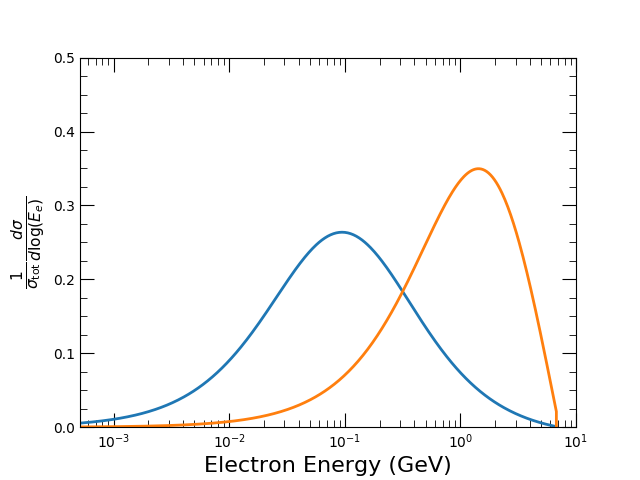
\includegraphics[width=0.8\textwidth]{figures/recoil_electron_spectrum.png}
\caption{Recoil electron spectrum for simple model.  The blue is for $m_{\gamma '}=10$ MeV, while the red is for $m_{\gamma '}=50$ MeV.  Both use values of $m_A=20$ GeV and $m_B=200$ MeV.}
\label{fig:recoil_spec}
\end{figure}

A fit was performed over this four-dimensional parameter space.  For each halo model, the number of expected signal events in each energy range at any particular point in parameter space is predicted by reweighting the signal MC discussed in \cref{sec:signal_mc}.   This reweighting accounts for the model dependent recoil electron energy spectrum, a well as the model dependent smearing between the boosted dark matter direction and the recoil electron direction.  A binned $\chi^2$ statistic was then computed similar to the one described above:
\begin{equation}
\chi^2(m_A,m_B,m_{\gamma '},\sigma_\textrm{tot})=\sum \limits_i^3 \min \limits_{\epsilon_i}\left[ 2  \left(  E_i-\mathcal{O}_i  + \mathcal{O}_i \ln \frac{ \mathcal{O}_i }{ E_i } \right)
             + \epsilon_i^2\right]
\end{equation}
where
\begin{equation}
E_i=b_i(1+\epsilon_i \sigma_i)+s_i.
\end{equation}
Note that there are 3 uncorrelated systematic errors representing the systematic uncertainty on the background estimate for each energy bin and no systematic uncertainty included for the signal.  A minimum $\chi^2$ over the whole 4-D parameter space was found, and the $\Delta \chi^2$ test statistic was defined as
\begin{equation}
\Delta \chi^2(m_A,m_B,m_{\gamma '},\sigma_\textrm{tot})=\chi^2(m_A,m_B,m_{\gamma '},\sigma_\textrm{tot})-\chi^2_\textrm{min}.
\end{equation} 
Note that the $\chi^2_\textrm{min}$ used here is different from the one found in \cref{eq:x2_min}.  Additionally, each halo model was considered separately so that there was a different minimum used for the Moore, NFW, and Kravtsov models, respectively.  For each halo model only a single search cone was considered, with the $5^\circ$ cone chosen for the Moore halo, the $10^\circ$ cone choosen for the NFW model, and the $40^\circ$ cone chosen for the Kravtsov model.  The choice of search cone for each model was made based on \cref{fig:opt_angle}.   Frequentist confidence regions could then be defined using toy MC.  A point in parameter space is considered excluded at confidence level $\alpha$ if less than (1-$\alpha$) of toy MC ensembles produced at the point resulted in a $\Delta \chi^2$ at the point greater than or equal to the value found from the data.   In these toy MC samples both statistical fluctuations and systematic fluctuations of the background were taken into account.

In \cref{sec:results}, confidence regions are presented for a baseline value of $m_{\gamma '}=20$ MeV in the plane $\sigma_\textrm{tot}/m_A^2$ vs $E_\textrm{max}$ where $E_\textrm{max}$ has been defined in \cref{eq:emax}.  The 4-D space $(m_A,m_B,m_{\gamma '},\sigma_\textrm{tot})$ is thus profiled down to a 3-D space $(E_\textrm{max},m_{\gamma '},\sigma_\textrm{tot}/m_A^2)$.  Since the boosted dark matter flux goes as $1/m_A^2$ (See \cref{eq:flux}), $\sigma_\textrm{tot}/m_A^2$ is proportional to the total signal event rate, and so all points in 4-D parameter space which are profiled onto the same point in 3-D parameter space will have very similar expected numbers of signal events.

The computation of confidence regions in the profiled space is performed as follows \cite{Olive:2016xmw}.  First, the set $U_{E_\textrm{max},\sigma_\textrm{tot}/m_A^2}$ is defined as the set of all values of $(m_A,m_B,\sigma_\textrm{tot})$ which correspond to $E_\textrm{max}$ and $\sigma_\textrm{tot}/m_A^2$.  Then the profile $\hat{\chi}^2$ and profile $\Delta \hat{\chi}^2$ are defined as:
\begin{equation}
\hat{\chi}^2(E_\textrm{max},m_{\gamma '},\sigma_\textrm{tot}/m_A^2)=\min \limits_{(m_A,m_B,\sigma_\textrm{tot})\in U_{E_\textrm{max},\sigma_\textrm{tot}/m_A^2}} \chi^2(m_A,m_B,m_{\gamma '},\sigma_\textrm{tot})
\end{equation}
\begin{equation}
\Delta \hat{\chi}^2(E_\textrm{max},m_{\gamma '},\sigma_\textrm{tot}/m_A^2)=\hat{\chi}^2(E_\textrm{max},m_{\gamma '},\sigma_\textrm{tot}/m_A^2)-\chi^2_\textrm{min}.
\end{equation}
A point $(E_\textrm{max},m_{\gamma '},\sigma_\textrm{tot}/m_A^2)$ is considered excluded at confidence level $\alpha$ if there is no point in $U_{E_\textrm{max},\sigma_\textrm{tot}/m_A^2}$ with the given value of $m_{\gamma '}$ for which more than or equal to (1-$\alpha$) of toy MC ensembles produced at the point result in a $\Delta \hat{\chi}^2$ greater than or equal to the one found in the data.






